\chapter{Method}

We took a systems design and implementation approach in our work, designing and implementing a working prototype system. Our plan of attack was formulated in accordance with the ultimate goal -- a working prototype system after 3 months of work. 

\section{Phases and design decisions}

The main project phases were
%
\begin{enumerate}

% Design phase
\item Phase: Design
\begin{enumerate}
\item Overall system design. Outline the concept and interaction of components.
\item Design of cryptographic protocols for authentication, re-keying and data transfer.
\item System components design
\begin{enumerate}
\item sensor prototype software.
\item sink and authentication server software.
\end{enumerate}
\end{enumerate}

% Crypto implementaiton phase
\item Phase: Implementation of cryptographic primitives
\begin{enumerate}
\item AES block cipher encryption and decryption
\item CBC-mode encryption and decryption
\item CMAC for authentication
\end{enumerate}

% System implementaiton phase
\item Phase: Implementation and integration
\begin{enumerate}
\item Authentication, re-keying and transfer protocol implementation
\item tsensor software development
\item sink and authentication server software development
\item System integration
\end{enumerate}

% Integration and testing
\item Phase: Unit and system tests in a test bed system

\end{enumerate}
%
Phases 2 and 3 overlapped in part. Unit tests (part of phase 4) were done continuously over the development cycle.


\subsection{System design decisions}

The main requirements for the TSense system were
%
\begin{enumerate}
\item The system should be as simple as possible, while at the same time giving reasonable security guarantees (confidentiality and integrity).
\item The cryptographic primitives should be as strong as possible, within the limits posed by the resource constrained sensor hardware.
\item All cryptographic algorithms should be open and non-proprietary.
\item System integrity should be ensured. In particular, an adversary should not be able to insert cloned sensors or simulate multiple sensors. 
\item The sensor should be as compact and cheap as possible.
\item The cryptographic software library for the sensor should be cross platform.
\end{enumerate}

\subsubsection{Simplicity}

Client/server systems are the simplest networked systems to design and implement. We decided upon this configuration for our test system. The client in this respect is a sensor/client pair, while the server is the sink. We decided to use a separate authentication server to allow for system scalability by deploying multiple sink servers; a single authentication server maintains the requirement that the secret device keys are distributed amongst the fewest nodes possible.

\subsubsection{Security}

We initially considered public key crypto algorithms, which would have allowed us to simplify the system further by excluding the authentication server. In such a system, each tsensor would hold a public/private keypair and the public key could be safely distributed amongst all sinks. Factoring and discrete logarithm based public key algorithms require very large keys -- 1024 bits at least for currently accepted security levels -- rendering this approach impractical on the ATmega328. 
%
%
However, elliptic curve public key cryptosystems \cite{koblitz1987,hankerson2004} require much shorter keys, on the order of the key lengths required for symmetric ciphers of comparable security.
%even as short as XXXX bits \cite{} \textbf{SEE ALSO \cite{NIST-recommended-elliptic-curves-1999}}, meaning that such algorithms may be practical on small resource constrained devices.  \textbf{CITE JOHNSON, HANKERSON.}
%

We decided to base our implementation solely on a single symmetric cryptographic primitive -- the AES block cipher. This approach saves the otherwise required coding and testing effort required in implementing an additional asymmetric algorithm. We therefore reserve the asymmetric cryptographic protocols for future work. However, note that the symmetric encryption algorithm is an important ingredient of asymmetric transport protocols, such as SSL; the much slower asymmetric algorithm is generally only used for symmetric key exchange, while the symmetric algorithm secures the data transfer itself. Thus the work done on this symmetric algorithm would still be of great use in any future work aimed at expanding this system to include an additional asymmetric algorithm.

%Security objectives are often stated in terms of the CIA trilogy -- \textit{confidentiality}, \textit{integrity} and \textit{availability}. 
%%
%Integrity is our primary concern. That is, no intermediary node, including the client holding the tsensor, should be able to modify messages (within computational bounds) undetected. Confidentiality is a secondary goal, but easily achieved by standard symmetric cryptographic primitives at tsensor and sink. Using such primitives, we can say that no active or passive adversary should be able (within computational bounds) to extract the transmitted information on the route between tsensor and sink.
%%
%We do not address availability issues -- denial-of-service, routing attacks and the like -- in our work.

\subsubsection{Open cryptographic algorithms}

Shannon's maxim "the enemy knows the system" is often a prudent assumption. Kerckhoffs' law\footnote{\textit{La cryptographie militaire}, Journal des sciences militaires, vol. IX, pp. 5--38, 161–191, 1883} states roughly the same principles, demonstrating the longevity of open design. Briefly, these assumptions dictate design principles where we assume any adversary, internal or external, knows intimately all aspects of the system, except for cryptographic keys. In particular, this includes knowledge of the algorithms and protocols employed. Layered security is certainly prudent in most practical scenarios, whereas reliance on security by obscurity is usually regarded as poor practice. We assume open cryptographic protocols in our design, basing the security solely on the secrecy of the shared private keys. For this reason, we selected the Rijndael block cipher \shortcite{fips-197-2001}, which was selected as the Advanced Encryption Standard (AES) in an open competition\footnote{\url{http://csrc.nist.gov/archive/aes}}.

\subsubsection{System integrity}

The Sybil attack \cite{Douceur2002} is a very real threat to any distributed system. In this attack, an adversary simulates multiple colluding nodes on a single (or relatively few) highly capable platform. An adversary could easily simulate thousands of tsensors on a single high-end PC, unless measures are taken to prevent such an attack. Cloning and multiple insertion of a single sensor is a related, but less damaging, attack.
%
Various solutions have been proposed for the Sybil attack, but the only absolute one is using strong and unforgeable node identities. This is the approach we take. Each tsensor has a strong and unforgeable (within computational bounds) identity in the form of a globally unique public ID and a 128-bit secret key (randomly generated), shared only with the authentication service. The identification and authentication protocol, described in Section~\ref{}, ensures (within computational bounds) that no more than one instance of any tsensor can be active in the system at any given time. Since the trusted authentication server holds the private keys and identities of all sensors manufactured, we can claim that no adversary can simulate a non-existent sensor.

System integrity requirements also dictate that the secret sensor keys should exist on as few nodes as possible. Each key is unique and permanently "burned" onto the tsensor device. The symmetric nature of the authentication protocol requires the key to be present on at least one other node. Minimal distribution of the secret key is achieved by using a trusted third party, the authentication server.

\subsubsection{Small and inexpensive sensor}

We base our sensor device on a small microcontroller, the Atmel ATmega328, widely used in sensor nodes and embedded applications. Our development platform is an Arduino Duemilanove experimentation board with an ATmega328 in a 28-pin DIL package. The board is about 5x7 cm in size.
The cost of this board is \$29.95 (+ shipping and import costs) in quantities of one from \url{http://www.sparkfun.com} in june 2010. 
%
A smaller surface mount package for the ATmega is available, which means that a production PCB for a trusted sensor may be as small as 2x2 cm. The sensor itself and tamperproof housing unavoidably adds to the size and cost, but a relatively small and inexpensive unit can be realized in a production setting.

\section{The TSense system}
\label{sec:tsense-system-overview}

\begin{figure}
\begin{center}
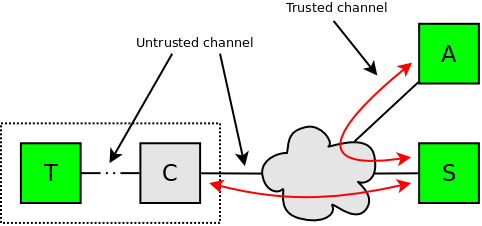
\includegraphics[width=0.6\textwidth]{figures/sys-overview.png} 
\end{center}
\caption{System overview. Interaction of the entities of the TSensor system. Green: Trusted entities. Gray: Untrusted entities (compromizable), Black channels: Untrusted, Red channels: Secure -- end-to-end encrypted and authenticated.}
\label{fig:sys-overview}
\end{figure}

The TSense system is shown in its simplest form in Figure~\ref{fig:sys-overview}. The module types are
%
\begin{description}

\item \textbf{T}: The trusted sensor -- \textit{tsensor} -- measures some array of quantities, e.g.\ temperature, pollutant particle count or luminosity, and publishes in an authenticated manner to a client ($C$). The published results may additionally be encrypted. tsensor would be a fully enclosed and tamper-proof unit in a production setting.

\item \textbf{C}: The client -- \textit{tsclient} -- hosts the sensor, e.g.\ physically attached or USB-connected. The client is the corruptible (adversary controlled) entity in our model. A honest client will always forward measurements unmodified to the sink $S$, whereas a corrupted $C$ may attempt modify the readings.

\item \textbf{S}: The sink server -- \textit{tsink} -- collects measurements forwarded from a number of client nodes over standard TCP/IP. A network may include multiple networked sinks to achieve some degree of scalability. In such a system, each of the sinks is a \textit{clusterhead} for a number of clients. In this work, we regard all sinks to be trusted. %This is a simplifying assumption that will be relaxed in future work.

\item \textbf{A}: The authentication server -- \textit{tauth} -- is the trusted third party (see Section~\ref{}) in our system and handles authentication of sensor/client pairs at the time of insertion into a working measurement network. 
%Even though we regard the $S$ to be trusted, it is a prudent measure to limit the distribution of sensor private keys. In our model, we limit the distribution of the private sensor keys to $T$ and $A$ nodes. 
We regard tauth to be incorruptible. A single tauth is assumed in the TSense system, which is a reasonable assumption from a scalability standpoint, since authentication takes place much less frequently than data collection.

\end{description}

Communications channels are as follows:
%
\begin{description}
\item {$tsensor \longleftrightarrow tsclient$:}
The tsensor and tsclient communicate over a serial link, provided by an USB-serial emulator. The tsclient, and by extension both of its communications channels, are considered untrusted. The tsensor and tsclient communicate using a dedicated serial communications protocol.

\item {$tsclient \longleftrightarrow tsink$:}
The tsclient and tsink communicate over an IP network, using a set of dedicated protocols described in Section~\ref{}. Other transport layer protocols than TCP may be used; our decision to use standard socket communications was merely one of convenience. 
%In particular, we may consider unreliable wireless communications protocols in our future work. 
tsclient and tsink use a standard unencrypted TCP connection; all security is provided by tsensor/sink operations, rendering critical operations inaccessible and unmodifiable (within computational bounds) by the untrusted tsclient and any third parties.

\item {$tsink \longleftrightarrow tauth$:}
The tsink and tauth communicate over an IP network, using TCP-IP and Transport Layer Security (TLS). TLS provides strong mutual authentication, confidentiality and integrity for message transfer between these two critical system components. Both have installed X.509 certificates and hold each others public keys.
%A bit of security-by-obscurity can be assumed by using non-standard ports.  

\end{description}

\section{Cryptographic primitives}
\label{sec:crypt-prim}

\subsection{The block cipher -- AES}
\label{sec:block-ciphher-aes}

A symmetric block or stream cipher is the workhorse of any confidentiality-preserving transfer protocol. 
%
Stream ciphers are generally faster than block ciphers, but harder to handle correctly. In particular, care must be taken to never re-use initialization vectors (IVs) when using stream ciphers. Examples of stream ciphers are e.g.\ found in the \textit{eCRYPT} stream cipher portfolio\footnote{\url{http://www.ecrypt.eu.org/stream}}. 
%
Suitable secure block ciphers include the industry-standard AES (Rijndael) \shortcite{fips-197-2001,daemen1999,daemen2000}, Blowfish \shortcite{schneier1997}, Skipjack \shortcite{skipjack-1998,brickell1993} and TEA/XTEA \shortcite{wheeler1995,needham1997}\footnote{See  \url{http://www.users.zetnet.co.uk/hopwood/crypto/scan/cs.html} for a more comprehensive list of suitable block- and stream ciphers.}.

We selected the Rijndael algorithm (AES), with the shorter 128-bit key length, for our prototype. This is the weakest AES variant, but the key length preserves valuable space on the \textit{tsensor} device. It is however quite strong enough for our purposes, since no known attacks exist against AES, except for reduced round (reduced strength) variants. One of the design requirements of the Rijndael algorithm was that it should be implementable on small 8-bit devices with limited memory. The algorithm has been implemented successfully on small devices, such as the YubiKey\footnote{\url{http://www.yubico.com/products/yubikey}} one time password generator.

We decided to write our own implementation of AES, rather than use an existing library. This choice was made in order to be able to support the various platforms in our system with the same code base. Our implementation of AES is close to the byte-oriented pseudocode published in the AES standard \shortcite{fips-197-2001}, although tuned for performance. More efficient implementations of AES are feasible using word oriented algorithms, in essence pre-computing the AES round functions in four lookup tables and reducing the encryption and decryption processes to four table lookups and XORs \cite[Section 5.2]{daemen1999}. However, such implementations depend on rather large lookup tables, a drawback for memory constrained devices. Further, such algorithms are highly architecture dependent and therefore tricky to write in a multi-platform manner. 
%We therefore decided to restrict our implementation to one close to the byte-oriented AES, although we take the advantage of long (32-bit) integers where possible.

We will denote encryption $C=\mathcal{E}_K(P)$ with a key $K$, on a plaintext (message) $P$, resulting in ciphertext $C$. Conversely, we use $P=\mathcal{D}_K(C)$ for decryption with a key $K$. For symmetric encryption, we have that $P=\mathcal{D}_K(\mathcal{E}_K(P))$.

Note that any secure block cipher and any mode of operation (as discussed in the following section) can be used in the TSense system. A particularly logical choice is to use the full strength AES-256, in case a higher security margin is desired, especially for the permanent device key.

\subsubsection{Mode of operation}

The AES block cipher, as all other block ciphers, can be used in several \textit{modes of operation} \shortcite{dworkin2001}. The most basic one, ECB, encrypts each block independently using the same shared key.  This leads to potential information leakage as identical plaintext encrypts to identical ciphertext, which may allow adversaries to determine correlations and perhaps deduce information. Stronger modes of operation generally feed parts of the plaintext or ciphertext into the encryption/decryption process for subsequent blocks, resulting in unpredictable variations, even for identical plaintext blocks. We used the Cipher Block Chaining (CBC) mode of encryption and decryption in our implementation \shortcite{dworkin2001}. The CBC mode of encryption is widely used, for example in the TinySec transport layer protocol \shortcite{karlof2004}, in conjunction with the Skipjack cipher.

The CBC-mode of operation can be used with any block cipher. For plaintext blocks $P_1, P_2, \dots, P_n$ and the corresponding cipertext blocks $C_1, C_2, \dots, C_n$, we have the encryption and decryption operations
\[
C_i = \mathcal{E}_K(P_i \oplus C_{i-1})
\]
and 
\[
P_i = \mathcal{D}_K(C_i) \oplus C_{i-1}
\]
where $C_0=IV$, an \textit{initialization vector}. 

\subsubsection{The initialization vector}

The initialization vector (IV) must be known to both the encrypting and decrypting parties and should be exchanged, at least periodically. Varying the IV ensures variation in cipertexts encrypted from identical plaintexts under the same key. The IV is not required to be secret, and can be sent in plaintext along with the message, but its integrity must be preserved, for example by encryption (secret IV) \shortcite[pp. 230]{menezes1996}. The IV must be unpredictable for use in CBC-mode \shortcite{dworkin2001}. One suitable method is to encrypt a nonce\footnote{Number used ONCE} under the same key as used for the encryption of the message plaintext. 

The nonces used in our protocol to prevent replays are generally secret; they also serve the purpose of providing variability in the produced ciphertext. Using these nonces as IV source is therefore not a satisfactory solution, as decryption would obviously be impossible. 
%
We propose the following compact method for IV generation. We choose a two byte random number, the IV nonce, which is included (in plaintext) in the standard message header (after the message ID). The IV nonce is encrypted (suitably padded) using a key derived from the encryption key being used to encrypt the present message. The 128-bit result is used as the IV for the message encryption and decryption. Using a short random nonce saves (potentially) on messaging costs but the tradeoff is the additional single key derivation and block encryption at both ends for each message exchange.
%
This method is in our opinion secure enough for our purpose, while being much simpler than that presented by \shortciteA{karlof2004} in their TinySec protocol.

%\url{http://en.wikipedia.org/wiki/Initialization_vector}
%\url{http://en.wikipedia.org/wiki/Cryptographic_nonce}
%\url{http://en.wikipedia.org/wiki/Salt_(cryptography)}
%\url{http://en.wikipedia.org/wiki/Key_derivation_function}

\subsubsection{Padding}

The smallest unit that a block cipher operates on is a single
block. The block size in AES is 16 bytes, hence the plaintext needs to
be padded if it isn't divisable by 16. We use the convention of
padding with a 1-byte followed by as few 0-bytes as possible ---
possibly none \cite[Appendex A]{dworkin2001}. That is, given the
datastring $x$ of length $n_x$, the padded string $x'$ is produced if
$16 \nmid n_x$, such that $16 \mid n_{x'}$. The lengths of the
encrypted sections in the protocol messages are either known
beforehand or the length is sent along in the message and this removes
the need of unambiqous padding.

There are other possible padding schemes. One example of such a scheme
is to pad the datastring $x$ with only 0-bytes to produce the padded
string $x'$ \cite[pp. 343]{menzes1996}. Another method is to pad the
string $x$ with $m$-bytes, where $m$ denotes the number of bytes needed to
pad the string to produce $x'$. \cite{RFC-2315-kaliski-1998}


\subsection{Message Authentication Code (MAC) algorithm}

Algorithms for generating \textit{message authentication codes (MACs)} are an important counterpart to symmetric ciphers. A MAC is an authentication tag which can be applied to a message, allowing the recipient to verify its authenticity in a cryptographically secure manner. Of course, both the sender and receiver must hold a shared key. The MAC tag is analogous to digital signatures, generated by public key signature algorithms. Common MAC algorithms include HMAC \shortcite{bellare1996}, which uses using cryptographically secure hash functions as its building block, and CBC-MAC \shortcite{bellare1999} and CMAC \shortcite{dworkin2005}, which are based on block ciphers. We chose CMAC (Cipher-based MAC), the stronger of the two, as our MAC algorithm and follow the guidelines of \shortciteA{rfc-4493-2006} and \shortciteA{rfc-4494-song-2006}. Choosing a block cipher based MAC algorithm means that we do not have to implement another primitive, such as a cryptographically secure hash function.

We denote MAC construction as $T=\mathcal{T}_K(M)$, for a key $K$. T is a tag (MAC) of the message $M$. Note that $M$ can be either plaintext or ciphertext.
MAC verification is a corresponding operation, in essence comparing the received MAC and message with an independently constructed MAC. That is, for a transmitted message $(M \parallel T)$, accept the received message $(M' \parallel T')$ as authentic if $\mathcal{T}_K(M') = T'$.

Note that any secure MAC algorithm and authenticating encryption mode, as described in the following section, can be used in the TSense system.

\subsubsection{Authenticating encryption}
\label{sec:authenc}

Authenticating encryption algorithms provide confidentiality and authenticity guarantees in a single primitive. In terms of block ciphers, we have several proposed authenticating modes of encryption, some examples being Counter with CBC-MAC (CCM) \shortcite{dworkin2004}, Offset Codebook (OCB) \shortcite{rogaway2003} and Galois Counter Mode (GCM) \shortcite{dworkin2007}. Authenticating stream ciphers are discussed by \shortciteA{teo2009}. However, in the TSense project, we use the conceptually simpler composition of generic encryption and MAC algorithms, as described by \shortciteA{bellare2007}.

According to \fullciteauthor{bellare2007}, generic encryption and MAC primitives can be composed in the following manner:
%
\begin{description}
\item \textbf{E\&M -- Encrypt-and-MAC}: Encrypt and MAC the plaintext separately and combine:\\ $\bar{\mathcal{E}}(K_e \parallel K_m,P) = \mathcal{E}_{K_e}(P) \parallel \mathcal{T}_{K_m}(P)$.
\item \textbf{MtE -- MAC-then-encrypt}: MAC the message, append to the plaintext and then encrypt:\\ $\bar{\mathcal{E}}(K_e \parallel K_m,P) =\mathcal{E}_{K_e}(P \parallel \mathcal{T}_{K_m}(P))$.
\item \textbf{EtM -- Encrypt-then-MAC}: Encrypt the message, MAC the ciphertext and append:\\ $\bar{\mathcal{E}}(K_e \parallel K_m,P) = C \parallel \mathcal{T}_{K_m}(C)$, where $C=\mathcal{E}_{K_e}(P)$.
\end{description}
%
Here, $\bar{\mathcal{E}}(K_e \parallel K_m,P)$ denotes authenticating encryption of a message $P$ using shared (symmetric) keys $K_e \parallel K_m$, where $K_e$ is the encryption key and $K_m$ is the MAC key. Two separate keys are required as re-using a key for two different purposes is considered a bad practice.

All three composition paradigms are strong enough for our purposes, since we use a block cipher and MAC for which no known (efficient) attacks exist. However, EtM is considered by \citeauthor{bellare2007} to be the strongest of the three and was therefore chosen as the composition paradigm for our cryptographic protocols.

\section{System components}

Our system consists of the four node types, previously introduced in Section~\ref{sec:tsense-system-overview}. We will now proceed to describe each module type independently in more details. Refer to the source code and documentation, available at the project site \url{http://code.google.com/p/tsense}, for further details.

\subsection{\textit{tsensor} -- Trusted sensor module}
\label{tsensor}

The tsensor gives us the ability to "bootstrap" trust in a networked measurement system, in which intermediary nodes, including the clients hosting the sensors, are untrusted. In order to provide this guarantee of trust, the tsensor cryptographically tags all readings with a message authentication code (MAC), providing receiver-end verifiability. The tsensor is intended to be a small, tamperproof device, guaranteeing that this trusted module or its produced results cannot be tampered with -- the physical protection\footnote{Our prototype is presently anything but tamperproof, as can readily be seen from Figure~\ref{fig:tsensor}. However, we assume a production model would be very well protected against physical tampering. Tamper-proof or tamper-resistant embedded systems are presently being produced by e.g.\ Freescale \url{http://www.freescale.com}.} prevents unauthorized access to the device internals, while the cryptographic protocols ensure (within computational bounds) that no adversary can modify or intercept messages. 

The requirements for the tsensor are
\begin{enumerate}
\item to measure some quantity and deliver securely to a trusted measurement sink (server).
\item to serve as a strong, unique and unforgeable identity for the platform to which it is attached (client).
\item to be as small and cheap as possible.
\end{enumerate}

Our choice of hardware for the tsensor prototype was in the spirit of these requirements. We choose the Atmel\footnote{\url{http://www.atmel.com}} ATmega series of CPUs, specifically an ATmega328 \cite{atmel-atmega-series-2010}. The ATmega328 is a RISC-based microprocessor, intended for embedded systems, capable of running at up to 20 MHz. It has 32K of on-board Flash program memory, 2K of RAM and 1K of EEPROM. Several digital I/O and analog inputs are provided. ATmega-series CPUs are widely used, for example in wireless sensor nodes \shortcite{akyildiz2002}.

We choose to use the Arduino Duemilanove\footnote{\url{http://arduino.cc/en/Main/ArduinoBoardDuemilanove}} prototyping board as our development platform in this project. The Duemilanove comes with an ATmega328 in a  28-pin DIL package and includes all the peripherals necessary for running the CPU. Additionally, a USB-to-serial converter is provided, allowing the board to be connected directly to a host computer for programming and data delivery.
%
The Duemilanove was augmented with a very simple sensor interface board, consisting of a couple of sensors (NTC thermistor and a photoresistor) and LEDs. The setup is shown in Figure~\ref{fig:tsensor}.
%

\begin{figure}[!t]
\centerline{
\subfigure[]{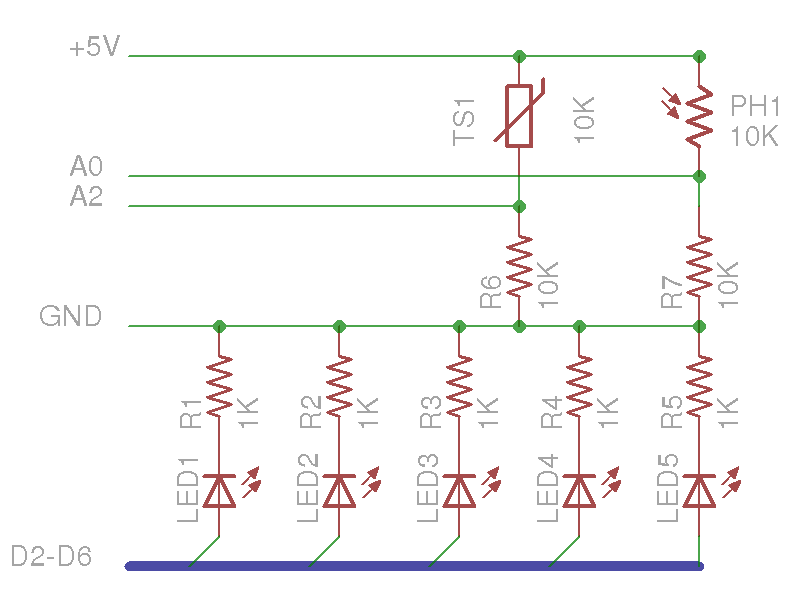
\includegraphics[width=0.45\textwidth]{figures/ts-schematic.png}
\label{fig:schematic}}
\subfigure[]{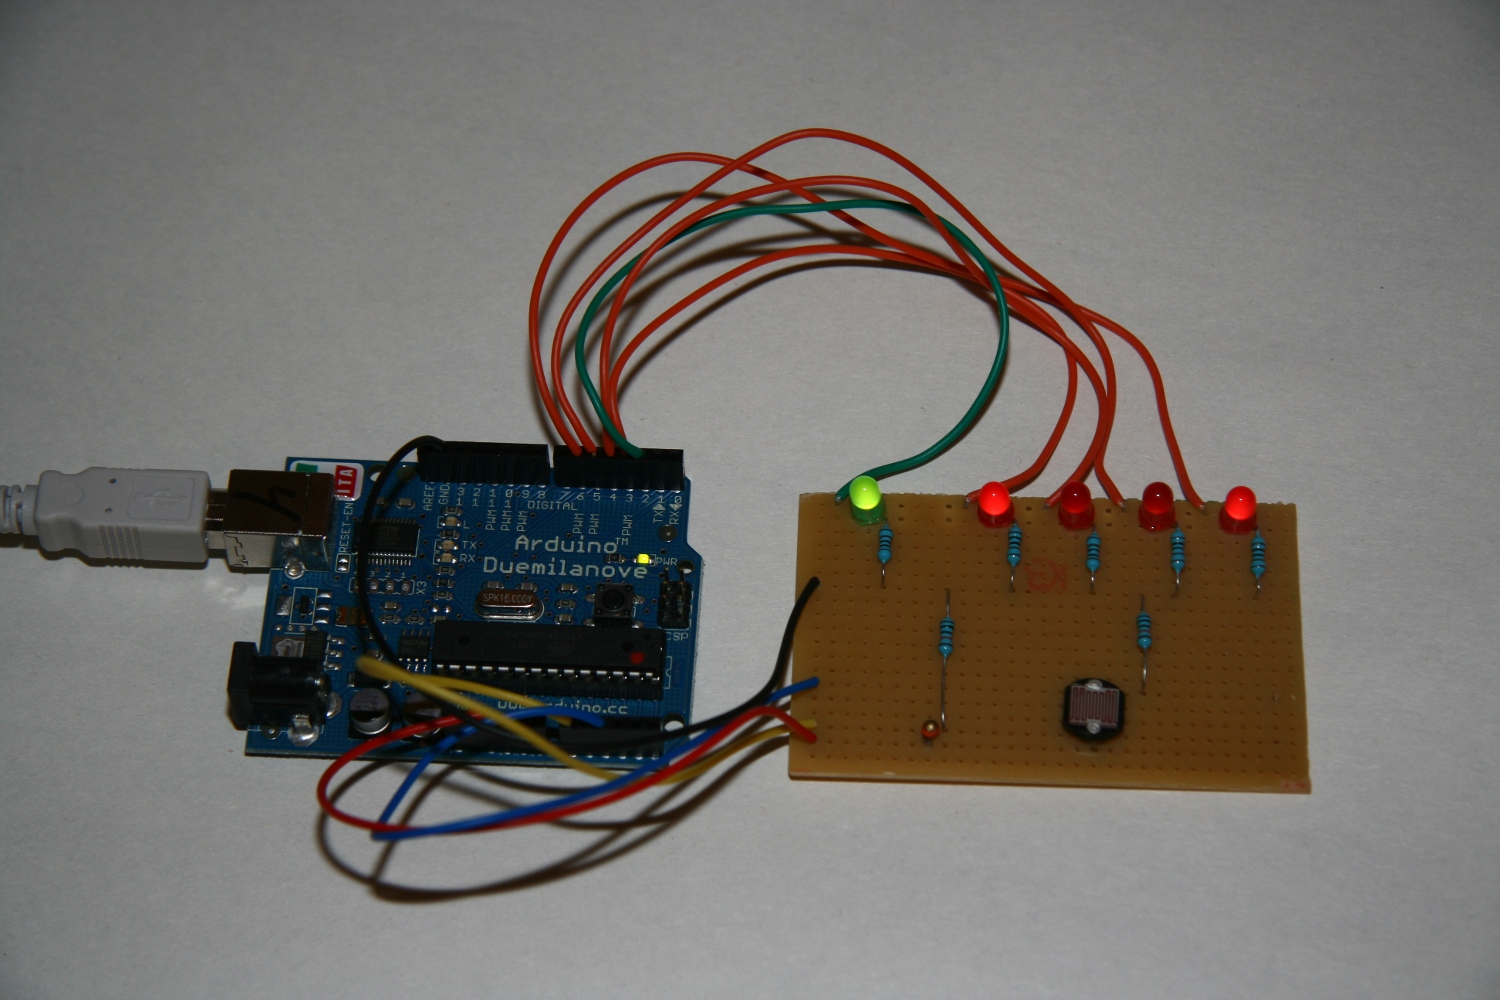
\includegraphics[width=0.45\columnwidth]{figures/tsensor.jpg}
\label{fig:picture}}} 
\caption{The tsensor prototype. 
\subref{fig:schematic} Schematic diagram of the sensor board. 
\subref{fig:picture} Picture of the Arduino and assembled sensor board.}
\label{fig:tsensor}
\end{figure}

\subsubsection{Software development} 
\label{tsensor-sdev}

The ATmega-series CPUs can be programmed in assembly language or using a C++ variant and the avr-gcc/avr-g++ compilers. The Arduino prototyping system includes an IDE for C/C++ development, with one button compile and upload capabilities, which we used for the tsensor software developmnt.

The 32K of program memory is rather restricted by current computing standards, but still allows development of fairly sophisticated programs. As stated previously, we chose an byte-oriented symmetric block cipher for all operations, rather than trying the limits of the hardware with a more computationally intensive asymmetric algorithm and digital signatures. We also implemented only one base cryptographic primitive -- the AES block cipher -- to conserve program memory space.

The 2K of RAM on the ATmega328 proved to be a more severe restriction. The RAM is needed to hold a small amount of operating system state, as well as the program heap and stack space. Our earliest tsensor prototypes were plagued by hard to diagnose spurious crashes, seemingly due to program memory corruption. The reason for these crashes was that allocating the AES lookup tables (s-box, inverse s-box and round-constant lookup tables), a total of 528 bytes, in RAM caused heap and stack memory collisions. We then moved all statically assigned data to the 1K EEPROM, which solved this particular problem.

We designed the software for maximum re-usability on the various system components. Concretely, the same implementation of AES in CBC mode and CMAC compiles for the ATmega328 on the tsensor and for 32- and 64-bit Intel/AMD platforms for the sink- and authentication server under Linux and OS X.

\subsubsection{Device identification data}

Each tsensor holds unique identifying information in its EEPROM. In a production device, this data would be unmodifiably "burned" into a ROM or a similar permanent storage device. The device data is as follows:
%
\begin{description}

\item \textbf{Public ID:} A 6-byte qlobally unique device identifier, consisting of a 2-byte manufacturer ID and a 4-byte device serial number. Note that the public ID can easily be expanded to any size in a production setting. The public device ID can as the name implies be freely disclosed to anyone. A command message issued by a client node over the serial line is used to retrieve this information.

\item \textbf{Private ID:} The private device ID is a 128-bit value, assigned by the manufacturer on assembly. The private ID is used as the initial encryption key $K_{AT}$ in the authentication protocol, as further described in Section~\ref{sec:cryptographic-protocols}. The private ID is assumed to be completely inaccessible on the tsensor device, although the symmetric nature of the system requires a copy to be kept by the trusted authentication service. The authentication component is further described in Section~\ref{sec:tsauthd-description}. The private ID is a 16-byte long random number, generated for each sensor.

\item \textbf{Manufacturer information:} (optional)
\begin{itemize}
\item Manufacturer name and address
\item device serial number
\item device manufacture date
\item software version
\end{itemize}
\end{description}

\subsubsection{Running the tsensor}

The tsensor receives its power through the USB-connection and is on while it is plugged in. It starts its operation in a standby mode that does not collect or provide any data. No data is provided by the sensor until the session and encryption keys have been successfully delivered, as described in Section~\ref{sec:cryptographic-protocols}.

\paragraph{External interface}

The tsensor interface board has a total of five LEDs. A green status LED blinks for standby and initialization modes and glows steadily in fully initialized execution mode. Four red LEDs are used to indicate intermediary authentication protocol states, data transfer operations and error states. The four red LEDs are not strictly necessary and may be omitted from a production sensor.

\paragraph{Serial API}

The sensor is controlled interactively through a set of control message which are issued by the client over the serial (USB) connection. This set of messages includes commands to set the sampling interval, sample buffer size and current time. 
%This is further described in \textbf{XXXX}. 
A vital security requirement of the tsensor serial API is that secret keys (permanent per-device private id, session or encryption keys) should ever be accessible, except indirectly they are used to encrypt outgoing information.

The most important feature of the serial API protocol is the device id request and response messages, which bootstrap the sensor into a working measurement system, as described in Section~\ref{sec:cryptographic-protocols}.

\subsubsection{tsensor utilities}

A set of utilities was developed to configure and diagnose the tsensor.

\paragraph{\textit{tsconfig}} is a utility for configuring a tsensor. The script is executed from the command line with a specified device public ID and "burns" the device EEPROM. This includes setting up the AES lookup tables, manufacturer information, public device ID and generating a \underline{fresh} 128-bit random private key. The utility \textit{generatekey} is used for the key generation and uses the Unix system random source \texttt{/dev/random} to generate random keys. \textit{tsconfig} and \textit{generatekey} are both part of the TSense code.

\paragraph{\textit{tsdiag}} extracts diagnostic information from a USB-connected tsensor device. All information accessible using the serial API is displayed. In the prototype, the entire EEPROM can be dumped, which breaks the basic security premise of the device -- the secret key is completely exposed. However, this feature is for development purposes only, and would be removed for a production device.

\subsection{\textit{tsclient} -- TSense client-side software}

The \textit{tsclient} is a small and completely untrusted software component installed on an equally untrusted hardware platform. The sole purpose of this software is to interface with the USB-connected tsensor and forward its messages to the sink server. The goal of this project is in essence to force this untrusted piece of software and the platform it resides on to provide only trustworthy information to the sink. 
%
We regard the attached tsensor to be strong enough to uniquely identify the client -- not as trusted but guarantees (within computational bounds) that the Sybil attack \shortcite{Douceur2002} is impossible in this system. In this sense, the tsensor functions similar to a SmartCard authentication system.

tsclient is written in python (v.\ 2.6), using the serial and socket libraries. Using a scripting language like Python for the client software is within the spirit of the project: the program is in plaintext on the client computer, allowing anyone to analyze and even modify it. No user written enhancements (or malicious tampering) should reduce the security guarantees of the overall system. We will attempt to support this claim in Section~\ref{sec:crypto-protocol-analysis}.

\subsubsection{Running tsclient}

tsclient is a python script, executed on the command line. See the source code documentation for details on command line switches. The user needs the connection information for the attached tsensor (USB connection string and baud rate) as well as for the sink server (IP address and port). On startup, the tsclient requests an partially encrypted and MACed identification package (see Section~\ref{sec:cryptographic-protocols-authentication}) which it then forwards (unmodified) to the designated sink server. This initial exchange bootstraps the authentication protocol and the insertion of the sensor/client pairing into a measurement system. After the initial device ID request, the tsclient is simply a proxy, forwarding encrypted messages unmodified back and forth between tsensor and sink. tsclient supports only a single tsensor and single sink in the current version. Future enhancements include supporting multiple sensors and multiple sinks per sensor for increased robustness.

\subsection{\textit{tssinkd} -- The TSense sink daemon}

\textit{tssinkd} -- The TSense sink daemon collects authenticated measurements from one or more tsensor client/sensor systems. In addition, it participates in the authentication and re-keying protocols, as is further described in Section~\ref{sec:cryptographic-protocols}.  For this purpose it uses the same AES encryption library developed for tsensor (see Sections \ref{sec:crypt-prim} and \ref{tsensor-sdev}) for encrypted communication between it and the tsensor.  The TSense sink server is a traditional Unix daemon written entirely in C++. It uses old school forking to service incoming requests on a child-per-request basis. Because of this the sink daemon needs a persistence layer to store state information. This state information consists of a sensor profile which contains the current session key of the sensor in question, an associated random key and the sensor's unique ID. Using these two keys the server can the generate the key schedules it need s to handle an incoming request. In addition to using a persistence layer to store sensor profiles the sink server  also requires a persistence layer to store measurement data collected from the various tsensor units it services.\\


The sink daemon software, it's persistence layer and the systems on which it resides are considered trusted for the purposes of this project. During implementation some corers were cut. As has already been mentioned communication with tsensor via the untrusted client is secure. Communication with the TSense authorization daemon (tsauthd) is, however, conducted over an industrial strength TLS tunnel (OpenSSL) with mutual authentication via x509 certificates. The persistence layer chosen, for the sake of speedy development, was MySQL since it is ubiquitous and well documented. Neither the persistence layer nor the database it self were secure or encrypted but for the purposes of this proof of concept system they are assumed to be secure. In a production environment the sink daemon would require a secure connection to an encrypted database, the sink daemon software and the machine it resides on would have to be located in a secure facility. Finally it would be advisable to switch from the MySQL library to a proper C++ based database abstraction layer. This should be fairly easy since care was taken to properly separate the sink server code from the database code so the transition to a new database library should be smooth.

\subsection{\textit{tsauthd} -- TSense authentication service}
\label{sec:tsauthd-description}

\textit{tsauthd} -- The TSense authentication daemon handles the integration of sensor/client pairs into a working measurement system. The authorization sever holds the private keys (private IDs) of every tsensor unit. Each tsensor must contact the authorization server via the untrusted client and the sink server to obtain a session key before the sensor can start persisting measurement data.  Much like sink server, the authorization server is a traditional Unix daemon written  entirely in C++ and uses old-school forking to handle requests on a child-per-request basis. All communication between the tsensor units and the authorization server is secure.  The authorization server uses the AES library developed for tsensor (see Sections \ref{sec:crypt-prim} and \ref{tsensor-sdev}) to communicate with tsensor but uses OpenSSL/TLS to communicate with the sink server. The authorization server uses the same persistence layer as the sink server to store device profiles consisting of the private key and unique ID of every tsensor in the system. The same caveats regarding the security of the persistence layer apply to the authorization server as did in the case of sink server.\\ 


As is the case with the sink server, the machine the authorization server resides on, the persistence layer the authorization server uses are considered to be highly a highly trusted and hardened purposes of this proof-of-concept project. In a production environment tsauthd would have to be deployed on a secure machine, connected to an encrypted database over a secure connection and it would have to be installed in a high security facility.

\section{Cryptographic protocols}
\label{sec:cryptographic-protocols}

% Was marked as TODO. Done?
Our protocol spans four parts; the authenticaion of the $tsensor$
device, the initial key exchange between it and $tssinkd$, subsequent
re-keying and the data transfers themselves. Messages are encrypted
with our AES-128 library and a CMAC of each ciphertext is appened to
every message for data integrety. The protocol aims to be as secure as
possible while still maintaing a small payload.

\subsection{Authentication and key exchange protocols}
\label{sec:cryptographic-protocols-authentication}

% Taka út? ↓
\textbf{See also \url{http://www.gsm-security.net/faq/gsm-authentication-key-generation.shtml} and \url{http://www.hackcanada.com/blackcrawl/cell/gsm/gsm-secur/gsm-secur.html} on the GSM network.}
% Removed '[B. Schneier -- Applied Crypto]'

The authentication protocol is a symmetric protocol using a trusted thrid party, based on the Needham-Schroeder authentication and key exchange protocol \shortcite{needham1978}. A modified Needham-Schroeder is also used in the Kerberos protocol \shortcite{neuman1994}. The main modification in our protocol is that $T$ does not communicate directly with $A$ but through $S$. This adds a layer of obscurity to $A$ as only the fairly well trusted $S$ needs direct knowledge of its address, in essence a bit of security-by-obscurity for $A$.
%
The original Needham-Schroeder was vulnerable to replay attacks \shortcite{denning1981}, which can be fixed by using nonces and/or timestamps \cite{needham1987}. We use both nonces and timestamps in our protocols.

As discussed in Section ~\ref{sec:authenc}, we use the \textit{Encrypt-then-MAC (EtM)} \shortciteA{bellare2007} composition paradigm, in which the plaintext is first encrypted and then a MAC of the ciphertext appended. We use $\mathcal{T}_K$ in our protocol to indicate \textit{tagging} (MACing) of the message ciphertext with a shared symmetric secret key $K$. $\mathcal{E}_K$ and $\mathcal{D}_K$ are used for encryption (resp.\ decryption) with a shared symmetric secret key $K$.

\subsubsection{Authentication}

The authentication and session key exchange proceeds as follows:

\[
C \rightarrow T: \textit{queryId}
\]
The client $C$ (untrusted) queries the sensor $T$ for its public ID.


\[
T \rightarrow C: (idrepsonse, T, \mathcal{E}_{TA,e}(T, N_T) \parallel \mathcal{T}_{TA,a})
\]

We denote a CMAC with $\mathcal{T}$ The keys $K_{TA,e}$ and $K_{TA,a}$
are both derived from $K_{TA}$.

The sensor $T$ returns its public id along with an encryption of both
the ID and a nounce $N_T$. We use the key $K_{TA,e}$ for
encryption. For authenticity, a CMAC of the message is then appended
to it. The nonce is only sent in encrypted form in this contrustion,
the purpose of it is to proved freshness and prevent replay attacks.

\[
C\rightarrow S: (idresponse,T,\mathcal{E}_{TA,e}(T,N_T) \parallel \mathcal{T}_{TA,a})
\]

$C$ passes the public id of $T$ and the encrypted packet to $S$.

\[
S \rightarrow A: (\mathcal{E}_{AS}(idresponse,T, \{
\mathcal{E}_{TA,e}(T,N_T) \parallel \mathcal{T}_{TA,a} \}) \parallel
\mathcal{T}_{AS,a})
\]

$S$ forwards the unmodified message from $T$ to $A$, which will then
read the encrypted packet, check the authenticity of it and repsond
accordingly. $S$ forwards the packet unmodified but adds extra security
by encrypting by a pairwise shared key $K_{AS}$ and the dirived key
$K_{AS,a}$. This is accomplished by using mutually authenticating TLS
to provide identification and authentication mechanism.

\subsubsection{Initial session key exchange}

If $T$ is accepted, then $A$ generates the session key $K_{ST}$ and
sends it to $S$, along with a rekeying timer $rt_{ST}$ and the
original nonce $N_T$.

\[
A \rightarrow S: (\mathcal{E}_{AS}(keytosink,T,K_{ST},rt_{ST}, \{
\mathcal{E}_{TA,e}(N_T,K_{ST},rt_{ST}) \parallel \mathcal{T}_{TA,a}
\} \parallel \mathcal{T}_{AS,a})
\]

%Hvernig er núna brugðvist við error?

$A$ will either deny or accept the authentication request or deny
it. If it accepts $T$ it will repsond with the randomly generates
session key $K_{ST}$ and a renewal timer $rt_{ST}$. The renewal timer
is a 2-byte integer which is decremented for each use of the session
key. $A$ also embeds a encrypted package for $T$, containing the
session key. It is MACed for authenticity. The shared symmetric key
$K_{AT}$ and the original nonce $N_T$ provides guarantees to $T$ that
it was in fact $A$ that generated this key.

If $T$ is denied it will repspond with \texttt{MSG\_T\_ERROR} (not yet
implemented).


\[
S \rightarrow C \rightarrow T: (keytosense,\mathcal{E}_{AT,e}(N_T,K_{ST},rt_{ST}) \parallel \mathcal{T}_{AT,a})
\]

$S$ forwards the encrypted package containing the nonce and session
key to $T$ through $C$. $T$ opens the package and retrieves
$K_{ST}$.

The session key $K_{ST}$ is a 16-byte long \textit{ephemeral} key from
wich $K_{ST,e}$ and $K_{ST,a}$ are derived. This makes cryptoanalytic
attacks unfeasable and limits the expousre of the key, because the
keys are used for a short period of time. \cite[pp. 494]{menzes1996}
. $rt_{ST}$ is the key renewal timer and $T$ will request a fresh key
when it reches zero.

The session key has now been delivered to $T$ and $S$ using
point-to-point key update with symmetric encryption.

\subsubsection{Subsequent session key exchanges}

The initial session key has now been delivered to $T$ and
$S$. Needham-Schroeder includes a handshake step in which the entities
receiving the session key make sure they both have the correct key. We
also use the handshake for the initial exchange of
encryption/authentication keys. These are the keys which are used in
the bulk of the crypto operations -- the data transfer itself.

The handshake must happen right after the delivery of $K_{ST}$ to $T$
and then the key-exchange is performed periodically to refresh the
encryption and authentication keys.

\[
T \rightarrow C \rightarrow S: (rekey,T,\mathcal{E}_{ST}(T,N_T) \parallel \mathcal{T}_{ST,a})
\]

Here $T$ uses the session key $K_{ST}$ to request a fresh key. A
guarantee of freshness is desired, but the hardware used for $T$ does
not have a hardware clock and we don't want to rely on $C$. So $N_T$
is a new nonce the will provide the key update with freshness. This is
done to provide bilateral implicit key authentication
\cite[pp.498]{menzes1996}.

In the first round, this message also serves to let $S$ know the
session key $K_{ST}$ was successfully delivered. The message code
\texttt{MSG\_T\_REKEY\_RESPONSE} is used for regular rekeying requests
and \texttt{MSG\_T\_REKEY\_HANDSHAKE} is used for the first-round handshake.

\[
S \rightarrow T: (newkey,T, \{ \mathcal{E}_{ST}(T,N_T,R,rt_{ST}) \parallel \mathcal{T}_{STe,a} \} )
\]

$S$ returns the new key material, a fresh 16-byte random number $R$ to
$T$.  $rt_{ST}$ is a fresh key renewal timer. When it reaches zero,
$T$ will request a fresh key. The encryption key is derived from
$K_{ST}$. This provides the bilateral implicit key authentication.

When the renewal timer $rt_{ST}$ reaches zero, $T$ will request a new
session key from $S$ using the current session key $K_{ST}$. It
follows the procedure described above.

Since the encryption and authentication keys $K_{TSe}$ and $K_{TSe,a}$
used for the actual traffic are short term \textit{ephemeral} keys,
they are only good for a very limited amount of traffic, say 10000
encryptions.

\subsection{Data transfer protocol}

The transfer protocol uses the encryption key $K_{ST,e}$ and authentication key $K_{ST,a}$
derived from the session key $K_{ST}$. The protocol is push-based.

\[
T \rightarrow C \rightarrow S: (\textit{data},T,length_{\mathcal{E}},\mathcal{E}_{ST,e}(T,t_T,D) \parallel \mathcal{T}_{STe,a})
\]
T encrypts the measurement data $D$, MACs it and delivers to
$C$, who will forward it to $S$. A fresh nonce $N_T$ prevents
replays.

The measurement data $D$ in on the following form:

\[
[ length_D \parallel m_1, m_2, \dots  m_n ]
\]

% mathbb?
where $length_D$ is the total length in bytes and $m_i \in \mathbb{Z}$ is a mesurment
record where $i \in \mathbb{N}$. 

\subsubsection{Finish message}

A well-behaved client should send a FINISH message when it wishes to
terminate a session. This message carries a summary of the session;
start time and end time of the sesson as well as the total number of
messages sent. This allows the sink to do some sanity checks. A FINISH
finish message will invalidate the current $S$-side session and
encryption keys as well as clean up resores.

% TODO: Reference the right section on the Sink
However, clients may leave without any notice and thus not sending the FINISH message. \textit{See section on the sink} for how $S$ state-keeping. 

Note: This refers to the key state only. Actual network connections
can be opened per transaction.

\subsection{Handling the unexpected}

The protocols outlined above assume well-behaved participants. This is
not necessarily the case. Timeouts, malfunctions, message losses,
malicious actions and program bugs are all factors to be considered
when designing robust protocols. We reserve most of the robustness
features for future work; components generally fail, hopefully
gracefully, in the current version when unexpected events
occur. However, we maintain a soft state for intermediary protocol
steps, allowing for some degree of robustness.

\subsection{Keys and key derivation}

%\textbf{\url{http://en.wikipedia.org/wiki/Key_derivation_function}}
%
%\textbf{\url{http://en.wikipedia.org/wiki/Key_strengthening}}
%
%\textbf{See \cite{ieee-1363-2000} on the KDF1 function.}

We observe the principle that a key should never be used for more than one purpose. For example, the same key is never used to encrypt and authenticate a message. We therefore always assume the existence of a key pair $(K_e,K_m)$ for encryption and authentication.
%
We have a number of such different key pairs -- private sensor ID (permanent master key), per-session generated session keys and limited lifetime encryption keys. For each of the encryption keys, we \textit{derive} corresponding authentication keys, using a suitable one-way function. A cryptographically secure hash function, such as sha-256, may be used for this purpose, but we elect to use our CMAC primitve. We assume an encryption key $K_e$ exists (permanent, generated or delivered) and we wish to derive the corresponding authentication (MAC) key. The derivation procedure is as follows:
\[
K_m = \mathcal{T}_\alpha(K_e)
\]
where $\mathcal{T}$ is a MAC generating function, $\alpha$ is a publicly available constant (128-bits) and $K_e$ is the encryption key used as \textit{key material} for the authentication key $K_m$. The encryption key is a "random-looking" series of bytes, which hashed by the MAC function produces a "random-looking" result. The one-wayness of the MAC function means that gaining knowledge of $K_m$ gives no information about $K_e$. The converse is of course not true, but an adversary gaining knowledge of $K_e$ breaks the initial premise for the derivation. 
%Cryptographically secure hash functions are usually used for this purpose and are cryptographically more sound than MACs. However, we feel that CMAC is at least strong enough for our purposes, especially for a proof-of-concept.

%\textbf{INTEGRATE:}
%The function $f$ can be a cryptographically secure hash function, in which case the derivation is essentially $K_a = f(K \parallel \alpha)$, similar to the key derivation function KDF1 in IEEE-1363-2000 \cite{ieee-1363-2000}. We have a keyed cryptographically secure hash function available, that is CMAC, so we might as well use that. In that case, we have $K_a = MAC_{\alpha}(K)$. $K$ is here the "key material" -- a base key or shared random value. In both cases, $\alpha$ is a pre-defined constant for each type of key produced. We can iterate the operation several times, similar to whats done in \shortcite{rsa-pkcs5-v2-1999}, but once is probably sufficient for our purposes. The output of the hash function or MAC is truncated down to the cryptographic key length. See also Menezes (ch. 13) on key derivation.

The keys and key derivation used are the following:
%
\begin{description}

\item $K_{TA}$ is the secret identity of the sensor $T$. It's unique for each sensor and shared only with $A$. An authenticity key is derived from $K_{TA}$: $K_{TA,a} = f_\alpha(K_{TA})$. The permanent secret keys are only used for initial authentication.
%\item $K_{AS}$ and $K_{AS,a}=f_\beta(K_{AS})$ are the shared keys for $S$ and $A$. For our purposes, we assume these keys to be handled by the TLS secure transportation layer.

\item $K_{ST}$ and $K_{ST,a}=f_\beta(K_{ST})$ are the session encryption and authentication keys, shared between a sink $S$ and sensor $T$. The key is generated (a random number is sufficient) by $A$ on successful identification of $T$. The session key is used only for re-keying.

\item $K_{STe}$ and $K_{STe,a}$ are the encryption and authentication keys for the data transfer protocol. They have a limited lifetime and must be replaced periodically by executing the re-keying protocol. The data transfer protocol does not deliver the key $K_{STe}$; rather, the \textit{key material} R (a 128-bit random number) is delivered. Key derivation is $K_{STe} = f_\gamma(R)$ and $K_{STe,a} = f_\varepsilon(K_{STe})$. 
%If authentication-only mode is used, we simply skip deriving the corresponding encryption key $K_{STe}$.
\end{description}
$\alpha$, $\beta$, $\gamma$ and $\varepsilon$ are publicly available 128-bit constants.

Note that the secure channel between sink and authentication server requires the key pair $(K_{AS},K_{AS,a})$. However, in our implementation, these keys are implicitly negotiated and derived by the TLS channel.

\subsection{Generation of cryptographic keys}

The system depends on one secret key -- the 128-bit private device ID $K_{TA}$ -- generated and burned to the device EEPROM at time of manufacture. This key is a 16-byte long random value, generated by reading from the \texttt{/dev/random} device in Unix. \texttt{/dev/random} allows access to an entropy pool, maintained by collecting environmental "noise" generated by the operating system and device drivers in normal operation. This is generally regarded as much closer to true randomness than pseudorandom generators, although vulnerabilities have been found in some implementations \shortcite{gutterman2006}. The non-blocking \texttt{/dev/urandom} can optionally be used for on-line key generation (session and transport keys) in the protocol to decrease latency.

%We regard the keys generated by reading /dev/random and /dev/urandom to be sufficiently random for our purposes. However, to reduce the risk of possible correlations, we propose to run the generated random number through a cryptographically secure hash function. In our case, we would use the CMAC primitive, in essence a keyed hash function, to generate the final key. One of the requirements for a robust MAC function is that the results are indistinquishable (within computational bounds) from a random value for any input. A hashed pseudorandom number will therefore be even more random than its predecessor. 

%Note that transport keys are derived from a 128-bit random number, in essence using the MAC method to add a layer of "randomness".

We provide an utility for generation of random cryptographic keys, \texttt{generatekey}. This utility is available along with the rest of the TSense code at the project code repository.

%\section{CHECK: Challenge-response authentication}
%
%See Bellovin and Merrit on EKE. Interesting C-R to simply encrypt a random number and requiring partner to echo back a re-encrypted decryption %of an encrypted random number. All encryptions-decryptions are done using a shared symmetric key -- the secret to be verified.
%
%Another method is to send a random number and require a hash of the random number with the secret to be verified. A MAC keyed on a shared secret key would be as effective.
%
%See \url{http://en.wikipedia.org/wiki/Challenge-response_authentication}
